{\bf Problem 2: Answer}

\begin{enumerate}[label={\arabic*.}]
    \item {\bf Yes}, because if there are multiple words per line then different words will be joined rather than their letters being joined. 
    \item {\bf No}, each additional iteration over the data produces a new BPE encoding. 
    \item See Figure 1 
	\begin{figure}[h!]
	    \centering
	    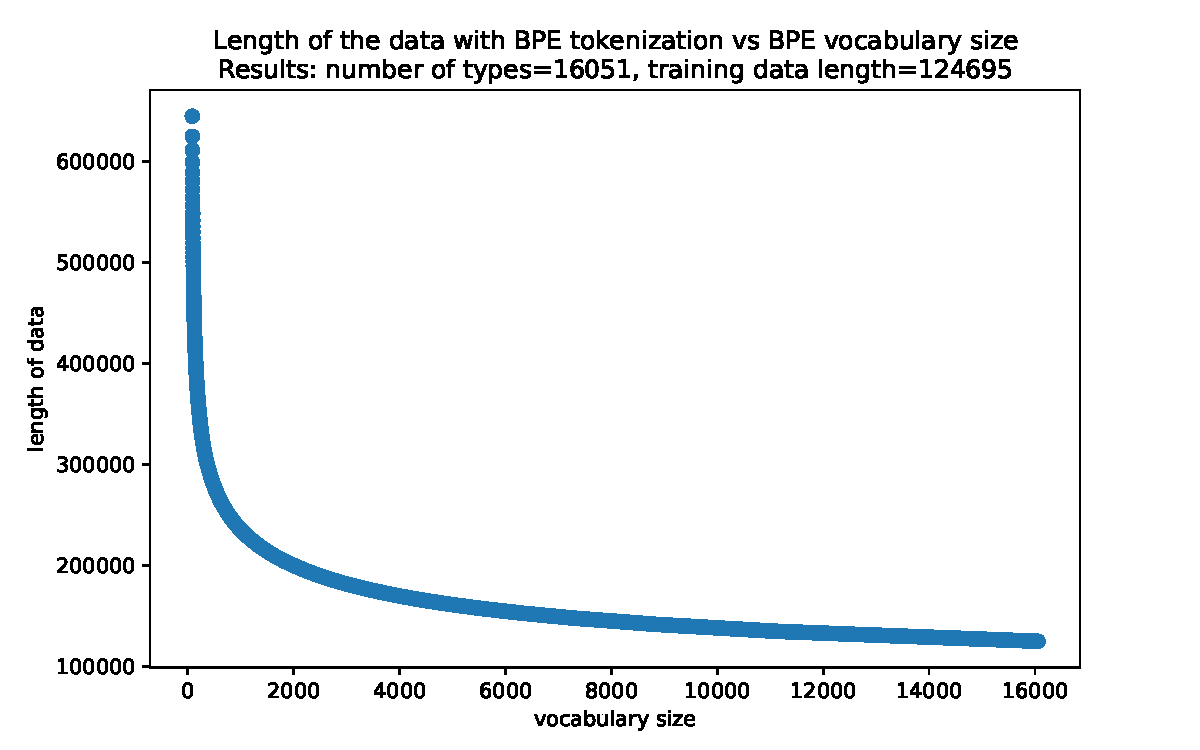
\includegraphics[width=0.8\linewidth]{../figures/plot.pdf}
	    \caption{}
	\end{figure}
    \item {\bf No}, we don't get any $<$unk$>$ tokens. We're unlikely to get $<$unk$>$ because that will only happen if the entire word cannot be encoded by BPE which will only occur if the sequence of letters composing that word hasn't been encoded during training. Using large, diverse training datasets reduces the likelihood of this occuring. 
	\begin{center}
	\begin{tabular}{ |c|c|c| } 
	    \multicolumn{3}{c}{Results of encoding 10 uncommon english words using BPE} \\	
	    \hline
	    & Word & Result \\
	    \hline
	    1 & fudgel & f ud g el$<$s$>$ \\
	    \hline
	    2 & nudiustertian & nu di ust er tian$<$s$>$ \\
	    \hline
	    3 & selcouth & sel cou th$<$s$>$ \\
	    \hline
	    4 & zabernism & z ab ern ism$<$s$>$ \\
	    \hline
	    5 & douceur & dou ce ur$<$s$>$ \\
	    \hline
	    6 & pauciloquent & pa uc il o qu ent$<$s$>$ \\
	    \hline
	    7 & defenestration & defen estr ation$<$s$>$ \\
	    \hline
	    8 & hiraeth & h ir ae th$<$s$>$ \\
	    \hline
	    9 & limerence & li mer ence$<$s$>$ \\
	    \hline
	    10 & sonder & s ond er$<$s$>$ \\
	    \hline
	\end{tabular}
    \end{center}
    \item Compared to this implementation of BPE, character encoding is quite fast since there are fewer comparisons. But it won't perform as well a BPE encoding because it's too fine grained and can't recognize word structures.
\end{enumerate}

{\bf Problem 2: Code}
\lstinputlisting[language=Python]{../code/p2.py}
